\documentclass[../main/main.tex]{subfiles}
\graphicspath{{./figures/}}

\makeatletter
\renewcommand{\@chapapp}{Travaux pratiques -- TP}
\makeatother

% \toggletrue{student}
\toggletrue{corrige}
% \renewcommand{\mycol}{black}
% \renewcommand{\mycol}{gray}

\hfuzz=5.002pt

\begin{document}
\setcounter{chapter}{25}

\settype{enon}
\settype{solu_prof}
\settype{solu_stud}

\chapter{\cswitch{%
	  Correction du TP
  }{%
	  Mesures de capacités thermiques
  }%
 }

\enonce{%
	\begin{tcn}*(exem)<ctc>"how"'t'{Capacités exigibles}
		\begin{itemize}
			\item Mettre en œuvre un protocole expérimental de mesure d'une grandeur
			      thermodynamique énergétique
		\end{itemize}
	\end{tcn}
	\vspace{-10pt}

	\section{Objectifs}

	\begin{itemize}
		\item Déterminer la capacité thermique d'un calorimètre.
		\item Utiliser la méthode des mélanges pour déterminer la capacité thermique
		      massique de différents matériaux.
		\item Sa familiariser avec une méthode de corrections de fuites thermiques.
	\end{itemize}

	\section{S'approprier}
	\subsection{Calorie et calorimètre}
	La calorie (symbole $\si{cal}$) est une ancienne unité de mesure exprimant une
	quantité d'énergie thermique (anciennement appelée «~chaleur~», mot qui vient
	lui-même de \textit{calor} en latin). Elle est définie comme étant la quantité
	d'énergie que l'on doit fournir à un gramme d'eau pour que sa température
	passe de \SI{15}{\degreeCelsius} à \SI{15}{\degreeCelsius}, à pression
	atmosphérique (\SI{1013}{hPa})~:
	\[
		\SI{1}{cal} = \SI{4.18}{J}
	\]
	\noindent
	\begin{minipage}[c]{.75\linewidth}
		\begin{itemize}
			\item Un calorimètre est un récipient à doubles parois de verre, entre
			      lesquelles on a fait un vide poussé.
			\item La surface de la paroi intérieure est argentée pour limiter les pertes
			      par rayonnement thermique.
			\item Le calorimètre est fermé par un couvercle permettant d'introduire un
			      agitateur, un thermomètre, une résistance chauffante.
		\end{itemize}
	\end{minipage}
	\hfill
	\noindent
	\begin{minipage}[c]{.20\linewidth}
		\begin{center}
			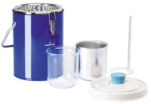
\includegraphics[width=\linewidth]{calo}
		\end{center}
	\end{minipage}
	\begin{itemize}
		\item Pour réaliser les expériences, on introduit dans le calorimètre soit
		      un vase en aluminium, soit un vase en verre.
		\item Le système est relativement bien isolé, et les échanges thermiques
		      avec l'extérieur sont très réduits.
		\item Le calorimètre est caractérisé par sa capacité thermique $C\ind{calo}$
		      (parois intérieures + instruments), ou par sa valeur en eau $\mu$
		      correspondant à la masse d'eau qui aurait la même capacité thermique que
		      le calorimètre~: on a donc $C\ind{calo} = \mu c\ind{eau}$, avec
		      $c\ind{eau} = \SI{4.18}{kJ.K^{-1}.kg^{-1}}$.
	\end{itemize}

	\begin{table}[htbp]
		\centering
		\caption{Valeurs de références de capacités thermiques massiques}
		\begin{tabularx}{.9\linewidth}{cYYYYY}
			\toprule
			\textbf{Matériau}                    &
			Eau liquide                          &
			Plomb                                &
			Cuivre                               &
			Fer                                  &
			Aluminium
			\\
			\midrule
			$\mathbf{c~(\si{J.K^{-1}.kg^{-1}})}$ &
			\num{4185}                           &
			\num{129}                            &
			\num{385}                            &
			\num{444}                            &
			\num{897}
			\\
			\bottomrule
		\end{tabularx}
		\label{tab:cref}
	\end{table}

	\subsection{Méthode des mélanges}
	Pour mesurer une capacité thermique massique \ftn{Aussi dite «~chaleur
		massique~» par abus.} inconnue d'un matériau solide, on réalise la
	\textbf{méthode des mélanges}~:
	\begin{itemize}
		\item on mesure les températures de tous les éléments du calorimètre, qui
		      sont normalement à la température de la pièce $\th_i$~;
		\item on insère une masse connue d'eau $m_1$ à température ambiante
		      $\th_i$~;
		\item on insère une masse connue $m_2$ de l'élément de chaleur massique
		      $c$ inconnue, à la température $\th_2$ connue
		\item à l'état d'équilibre final, le calorimètre, les masses $m_1$ et
		      $m_2$ sont à la même température $\th_f$.
	\end{itemize}

	\subsection{Prise en compte des fuites~: méthode de \textsc{Regnault}}
	Aucune transformation n'est rigoureusement adiabatique. Des échanges de
	chaleur parasites entre le calorimètre et le milieu extérieur ont lieu. Ils
	suivent en première approximation la loi de \textsc{Newton}~:
	\[
		\delta Q = kS (\th\ind{calo} - \th\ind{ext})\dd{t}
	\]
	avec $\delta Q$ la variation infinitésimale de transfert thermique, $k$ un
	coefficient, $S$ la surface de contact, $\th$ les températures en
	\si{\degreeCelsius} et $t$ le temps.
	\smallbreak
	Il existe plusieurs méthodes pour tenter de corriger l'erreur systématique
	due à ces échanges de chaleur. La correction la plus courante est celle de
	\textsc{Regnault}.
	\smallbreak
	\noindent
	\begin{minipage}[c]{.45\linewidth}
		\begin{itemize}
			\item On met un capteur de température dans le calorimètre, afin de
			      mesurer la température à intervalles de temps réguliers.
			\item L'évolution de la température est modélisée par des droites,
			      représentées ci-contre.
			\item On modélise les mesures par 3 portions de droites (1), (2) et
			      (3). On trouve alors les instants $t_1$ et $t_2$.
		\end{itemize}
	\end{minipage}
	\hfill
	\noindent
	\begin{minipage}[c]{.53\linewidth}
		\begin{center}
			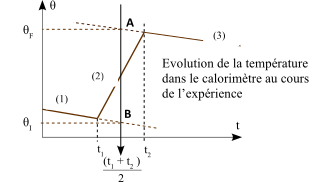
\includegraphics[width=\linewidth]{regnault}
		\end{center}
	\end{minipage}
	\begin{itemize}
		\item On trace ensuite la droite verticale d'équation $t =
			      (t_1+t_2)/2$, dont l'intersection avec les droites (1) et (3)
		      donne les points A et B, d'ordonnées $\th_i$ et $\th_f$.
		\item $\mathbf{\th_f - \th_i}$ \textbf{représente la véritable
			      variation de température du calorimètre à utiliser dans le bilan
			      enthalpique adiabatique}.
	\end{itemize}
	\begin{center}
		\begin{tcn}(impo){Attention}
			Pour réaliser de telles courbes, il faut \textbf{commencer les
				mesures environ \SI{5}{minutes} avant l'introduction du corps
				chaud et continuer environ \SI{10}{minutes} à partir de la
				décroissance de la température}.
		\end{tcn}
	\end{center}
}%

\setcounter{section}{3}
\section{Analyser~: méthode des mélanges}
\setlist[blocQR,1]{leftmargin=10pt, label=\clenumi}
\QR{%
	On considère le système \{calorimètre, $m_1$, $m_2$\}. Montrer que
	$\Delta{H}\ind{sys} = 0$.
}{%
	$Q = 0$ et $W_u = 0$, donc $\Delta{H} = Q + W_u = 0$.
}%
\QR{%
	En déduire une expression de $c$ en fonction de $m_1$, $m_2$, $\mu$,
	$c\ind{eau}$, $\th_i$, $\th_2$ et $\th_f$.
}{%
	solu
}%

\section{Réaliser}
\subsection{Mesures directes}
\QR{%
	Proposer un protocole expérimental utilisant la méthode des mélanges pour
	mesurer les capacités thermiques massiques $c$ du plomb, du cuivre, du fer et
	de l'aluminium.
}{%
	solu
}%

\enonce{%
	\begin{tcn}(expe)<itc>{Mesures directes}
		\begin{itemize}
			\item Réaliser l'expérience correspondant au protocole proposé. Attention à se
			      placer dans des conditions expérimentales pour lesquelles l'écart de
			      température $\th_f - \th_i$ est suffisamment important.
			\item Il faut agiter régulièrement durant la mesure pour s'assurer de
			      conserver une température homogène.
		\end{itemize}
	\end{tcn}
}%

\resetQ
\setlist[blocQR,1]{leftmargin=10pt, label=\sqenumi}
\QR{%
	Recopier et compléter le tableau suivant sur vos comptes-rendus. Calculer les
	valeurs de $c\ind{matériau}$, $u(c\ind{matériau})$ et $E_N$ sur
	\texttt{Capytale} à l'adresse
	\url{https://capytale2.ac-paris.fr/web/c/00a2-3541233}, grâce à une
	propagation des incertitudes par méthode \textsc{Monte-Carlo}. Vous utiliserez
	un \texttt{DataFrame} du module \texttt{pandas} pour visualiser votre tableau
	\texttt{Python} avant de recopier les valeurs. \textbf{Pas de calculatrice en
		vue~!}
	\begin{center}
		\begin{tabularx}{\linewidth}{cYYYYYYY}
			\toprule
			\textbf{Matériau}                        &
			$\th_i \pm u(\th_i)$                     &
			$\th_2 \pm u(\th_2)$                     &
			$\th_f \pm u(\th_f)$                     &
			$m_1 \pm u(m_1)$                         &
			$m_2 \pm u(m_2)$                         &
			$c\ind{matériau} \pm u(c\ind{matériau})$ &
			$E_N$
			\\
			\midrule
			$\vdots$                                 &
			$\vdots$                                 &
			$\vdots$                                 &
			$\vdots$                                 &
			$\vdots$                                 &
			$\vdots$                                 &
			$\vdots$                                 &
			$\vdots$
			\\
			$\vdots$                                 &
			$\vdots$                                 &
			$\vdots$                                 &
			$\vdots$                                 &
			$\vdots$                                 &
			$\vdots$                                 &
			$\vdots$                                 &
			$\vdots$
			\\
			\bottomrule
		\end{tabularx}
	\end{center}
}{%
	solu
}%
\QR{%
	Commenter vos résultats de mesures en comparaison aux valeurs de référence du
	Tableau~\ref{tab:cref}.
}{%
	solu
}%

\subsection{Mesures avec \texttt{LatisPro}}
\enonce{%
	Le tracé de la courbe d'évolution de la température dans le calorimètre $\th =
		f(t)$ se fait automatiquement par l'intermédiaire d'une sonde de température
	reliée à l'interface \texttt{Sysam} de l'ordinateur et au logiciel
	\texttt{LatisPro}.
	\begin{tcn}(expe)<itc>{Mesures avec fuites}
		\begin{itemize}
			\item Ôter le thermomètre du calorimètre et le remplacer par la sonde
			      thermique reliée à la carte d'acquisition \texttt{Sysam}.
			\item Renseigner les réglages suivants
			      \begin{itemize}
				      \item Mode~: température
				      \item Durée d'acquisition~: \SI{900}{s}
				      \item Nombre de points~: \num{100}
			      \end{itemize}
			\item Prendre soin de respecter le temps de mesure avant et après
			      l'insertion comme indiqué dans la partie «~S'approprier~».
		\end{itemize}
	\end{tcn}
}%

\setlist[blocQR,1]{leftmargin=10pt, label=\clenumi}
\QR<[start=4]>{%
	Adapter le protocole expérimental précédent utilisant la méthode des mélanges
	pour mesurer les capacités thermiques massiques en utilisant la méthode de
	\textsc{Regnault}.
}{%
	solu
}%

\resetQ
\setlist[blocQR,1]{leftmargin=10pt, label=\sqenumi}
\QR<[start=3]>{%
	Reprendre les mesures dans un \textbf{nouveau tableau}, toujours à l'aide de
	\texttt{Capytale}.
	\begin{center}
		\begin{tabularx}{\linewidth}{cYYYYYYY}
			\toprule
			\textbf{Matériau}                        &
			$\th_i \pm u(\th_i)$                     &
			$\th_2 \pm u(\th_2)$                     &
			$\th_f \pm u(\th_f)$                     &
			$m_1 \pm u(m_1)$                         &
			$m_2 \pm u(m_2)$                         &
			$c\ind{matériau} \pm u(c\ind{matériau})$ &
			$E_N$
			\\
			\midrule
			$\vdots$                                 &
			$\vdots$                                 &
			$\vdots$                                 &
			$\vdots$                                 &
			$\vdots$                                 &
			$\vdots$                                 &
			$\vdots$                                 &
			$\vdots$
			\\
			$\vdots$                                 &
			$\vdots$                                 &
			$\vdots$                                 &
			$\vdots$                                 &
			$\vdots$                                 &
			$\vdots$                                 &
			$\vdots$                                 &
			$\vdots$
			\\
			\bottomrule
		\end{tabularx}
	\end{center}
}{%
	solu
}%
\QR{%
	Commenter vos résultats de mesures en comparaison aux valeurs de référence du
	Tableau~\ref{tab:cref}.
}{%
	solu
}%
\end{document}
